\chapter{Eigenvalues and Eigenvectors}
In Chapter "Eigenvalues and Eigenvectors," Section 1 comprehensively introduced and explored these foundational concepts within finite matrices, emphasizing methodologies, practical applications, and significance. Transitioning to Section 2, the analysis extended to eigenvalues and eigenvectors in infinite matrices. This involved solving characteristic equations with determinant and identity matrix, incorporating computational intricacies such as exponentiation and logarithmic transformations. The systematic process for discerning each eigenvalue and its corresponding eigenvector provided valuable insights into the intrinsic properties of the infinite matrix.
\section{Eigenvalues and eigenvectors of finite matrices}\label{sec:intro_eigen}
\begin{definition}
Let $ A $ be an $ n \times n $ matrix, and let $ {X} \in \mathbb{C}^n $ be a nonzero vector for which
\begin{center}
    $A{X} = \lambda {X} $
\end{center}
for some scalar $ \lambda $. Then $ \lambda $ is called an eigenvalue of the matrix $ A $, and $ {X} $ is called an eigenvector of $ A $ associated with $ \lambda $, or a $ \lambda $-eigenvector of $ A $.\newline
The set of all eigenvalues of an $ n \times n $ matrix $ A $ is denoted by $ \sigma(A) $ and is referred to as the spectrum of $ A $.\cite{gilbertstrang}    
\end{definition}

\begin{example}
    Find the eigenvalues of the matrix \[ A = \begin{bmatrix} 2 & 2 \\ 5 & -1 \end{bmatrix} \].

The eigenvalues are those \( \lambda \) for which \( \text{det}(A - \lambda I) = 0 \). Now 
$$
\begin{aligned}
\operatorname{det}({A}-\lambda {I}) & =\operatorname{det}\left(\left[\begin{array}{cc}
2 & 2 \\
5 & -1
\end{array}\right]-\lambda\left[\begin{array}{ll}
1 & 0 \\
0 & 1
\end{array}\right]\right) \\
& =\operatorname{det}\left(\left[\begin{array}{cc}
2 & 2 \\
5 & -1
\end{array}\right]-\left[\begin{array}{cc}
\lambda & 0 \\
0 & \lambda
\end{array}\right]\right) \\
& =\left|\begin{array}{cc}
2-\lambda & 2 \\
5 & -1-\lambda
\end{array}\right| \\
& =(2-\lambda)(-1-\lambda)-10 \\
& =\lambda^2-\lambda-12 .
\end{aligned}
$$



The eigenvalues of \( A \) are the solutions of the quadratic equation \( \lambda^2 - \lambda - 12 = 0 \), namely \( \lambda_1 = -3 \) and \( \lambda_2 = 4 \).

As we have discussed, if \( \text{det}(A - \lambda I) = 0 \), then the equation \( (A - \lambda I)x = b \) has either no solutions or infinitely many. When we take \( b = 0 \), however, it is clear by the existence of the solution \( x = 0 \) that there are infinitely many solutions (i.e., we may rule out the "no solution" case). If we continue using the matrix \( A \) from the example above, we can expect nonzero solutions \( x \) (infinitely many of them, in fact) of the equation \( Ax = \lambda x \) precisely when \( \lambda = -3 \) or \( \lambda = 4 \). Let us proceed to characterize such solutions.

First, we work with \( \lambda = -3 \). The equation \( Ax = \lambda x \) becomes \( Ax = -3x \). Writing \( x = \begin{bmatrix} x_1 \\ x_2 \end{bmatrix} \) and using the matrix \( A \) from above, we have 
\[
\begin{aligned}
    Ax &= \begin{bmatrix} 2x_1 + 2x_2 \\ 5x_1 - x_2 \end{bmatrix}, \\
    -3x &= \begin{bmatrix} -3x_1 \\ -3x_2 \end{bmatrix}.
\end{aligned}
\]
Setting these equal, we get
$$
\begin{aligned}
{\left[\begin{array}{c}
2 x_1+2 x_2 \\
5 x_1-x_2
\end{array}\right]=\left[\begin{array}{c}
-3 x_1 \\
-3 x_2
\end{array}\right] } & \Rightarrow 2 x_1+2 x_2=-3 x_1 \quad \text { and } \quad 5 x_1-x_2=-3 x_2 \\
& \Rightarrow 5 x_1=-2 x_2 \\
& \Rightarrow x_1=-\frac{2}{5} x_2 .
\end{aligned}
$$

This means that, while there are infinitely many nonzero solutions (solution vectors) of the equation ${A x}=-3 {x}$, they all satisfy the condition that the first entry $x_1$ is $-2 / 5$ times the second entry $x_2$. Thus all solutions of this equation can be characterized by
$$
\left[\begin{array}{c}
2 t \\
-5 t
\end{array}\right]=t\left[\begin{array}{c}
2 \\
-5
\end{array}\right]
$$

 where \( t \) is any real number. The nonzero vectors \( x \) that satisfy \( Ax = -3x \) are called eigenvectors associated with the eigenvalue \( \lambda = -3 \). One such eigenvector is \( u_1 = \begin{bmatrix} 2 \\ -5 \end{bmatrix} \), and all other eigenvectors corresponding to the eigenvalue \((-3)\) are simply scalar multiples of \( u_1 \) i.e. \( u_1 \) spans this set of eigenvectors.

Similarly, we can find eigenvectors associated with the eigenvalue \( \lambda = 4 \) by solving \( Ax = 4x \)
\[
\begin{aligned}
    \begin{bmatrix} 2x_1 + 2x_2 \\ 5x_1 - x_2 \end{bmatrix} &= \begin{bmatrix} 4x_1 \\ 4x_2 \end{bmatrix} 
    &\Rightarrow 2x_1 + 2x_2 = 4x_1 \text{ and } 5x_1 - x_2 = 4x_2 
    &\Rightarrow x_1 = x_2.
\end{aligned}
\]

Hence, the set of eigenvectors associated with \( \lambda = 4 \) is spanned by \( u_2 = \begin{bmatrix} 1 \\ 1 \end{bmatrix} \).
\end{example}
\subsection{Should we add?}
For a real matrix, the logarithm exists if and only if all its eigenvalues are positive. Specifically, the logarithm of a real matrix $A$ exists if and only if $A$ is positive definite, meaning that all its eigenvalues are strictly positive.\newline

In the provided MATLAB \ref{lst:matrices-real-number} code, the attempt to generate a matrix with positive real eigenvalues is essential to ensure that the logarithm calculation using the series expansion is meaningful and converges to a valid result.

Generated matrix with positive real eigenvalues and norm($I$ - $A$) $< 1$ after $261$ attempts.

Original Matrix $A$:
\[ A =
    \begin{bmatrix}
        1.3072 & 0.3070 & -0.4733 \\
        -0.0204 & 0.3143 & 0.3128 \\
        -0.5614 & 0.1224 & 0.9682
    \end{bmatrix}
\]

Eigenvalues of $A$:
\[
    \begin{bmatrix}
        1.6492 \\
        0.7691 \\
        0.1715
    \end{bmatrix}
\]

Norm of $(I-A)$: 0.929513

Original matrix determinant (up to 10 decimal places): 0.2175165714

Approximated determinant after 98 iterations: 0.2175165715

Final Determinant Error: 0.0000000001

\[
    \begin{bmatrix}
        0.1199 & 0.6028 & -0.5924 \\
        0.1597 & -1.3680 & 0.6558 \\
        -0.5730 & 0.4526 & -0.2773
    \end{bmatrix}
\]\newline
 A complex matrix has a logarithm if and only if it is invertible. The logarithm is not unique, but if a matrix has no negative real eigenvalues, then there is a unique logarithm that has eigenvalues all lying in the strip $\{z \in \mathbb{C} \ \vert \ -\pi < \textit{Im} \ z < \pi\}$. This logarithm is known as the principal logarithm.

The answer is more involved in the real setting. A real matrix has a real logarithm if and only if it is invertible and each Jordan block belonging to a negative eigenvalue occurs an even number of times. If an invertible real matrix does not satisfy the condition with the Jordan blocks, then it has only non-real logarithms. This can already be seen in the scalar case: no branch of the logarithm can be real at -1. The existence of real matrix logarithms of real $2 \times 2$ matrices is considered in a later section.




Generated complex matrix with eigenvalues in the strip and norm less than $1$ after $401$ attempts.

Original Complex Matrix $A$:
\[
\begin{bmatrix}
   0.3145 - 0.6665i & -0.1452 - 0.1428i \\
   0.0042 - 0.0410i & 1.0970 + 0.4197i
\end{bmatrix}
\]

Eigenvalues of $A$:
\[
\begin{bmatrix}
   0.3140 - 0.6727i \\
   1.0975 + 0.4259i
\end{bmatrix}
\]

Original matrix determinant:
\[
0.6311 - 0.6045i
\]

Approximated Logarithm of $A$ using series expansion:
\[
\begin{bmatrix}
  -0.2998 - 1.1272i & -0.1079 - 0.2115i \\
   0.0198 - 0.0439i & 0.1650 + 0.3631i
\end{bmatrix}
\]

$\text{exp(trace}(\text{Log}A))$:
\[
0.6309 - 0.6046i
\]
\begin{center}
   \begin{figure}
    \centering
    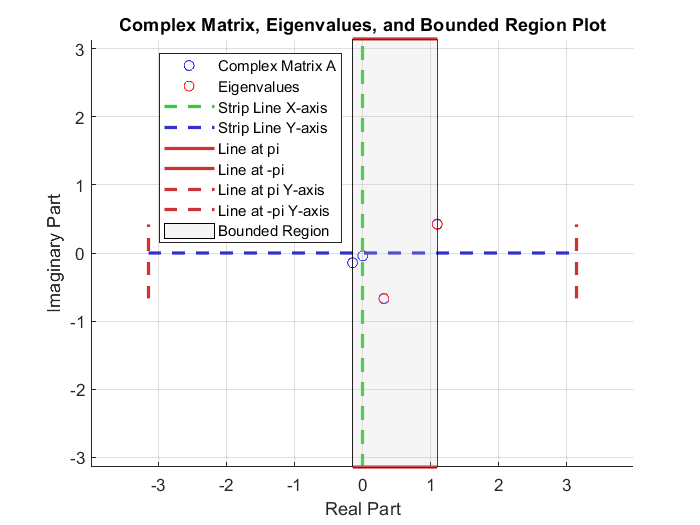
\includegraphics[width=0.8\linewidth]{Figures/eeeeeeeeeeeeeeeeeee.png}
    \caption{logarithm of complex matrix}
    \label{fig:complex}
    \end{figure} 
\end{center}

This graph\ref{fig:complex} shows the complex matrix elements, eigenvalues, and bounded region plot. It is a way of visualizing the properties of complex matrices and their eigenvalues. The eigenvalues are the blue crosses on the graph, and they are the solutions of the characteristic equation of the matrix. The unit circle is the blue dashed circle, and it is the set of complex numbers with magnitude one. The bounded region is the shaded area, and it is the region where the matrix norm is less than one. The strips and lines are related to the convergence and divergence of the matrix power series. This graph is part of an application that allows you to explore infinite matrices and their results.
\section{Eigenvalues and eigenvectors of infinite matrices }
We will try to determine the eigenvalues and eigenvectors of the infinite matrix by solving a characteristic equation
\[
\text{det}(A - \lambda I) = 0.
\]
So, we have to calculate
\[
\text{det}(A - \lambda I) = \exp(\text{tr}(\log(A - \lambda I))),
\]
where \(\text{tr}(\log(A - \lambda I))\) is a convergent series. For an  eigenvalue \(\lambda\), we find the corresponding eigenvector \(v = (x_1, x_2, x_3, \ldots)\) from the system of equations:
\[
(A - \lambda I) \begin{bmatrix} x_1 \\ x_2 \\ x_3 \\ \vdots \end{bmatrix} = \begin{bmatrix} 0 \\ 0 \\ 0 \\ \vdots \end{bmatrix}.
\]  
\begin{sourcecode}
\label{sourcecode-matrix-inverse}  
    \begin{lstlisting}[language=MATLAB, caption=finding determinant equation using eigen value]function log_eigen_det()
    number_of_terms = 1000;
    tolerance = 1e-4;  % Set the desired threshold for convergence
    
    if nargin < 1
        matrixSize = 2;
        A = randn(matrixSize);

        % Counter for attempts to generate matrix with positive real eigenvalues
        attemptCount = 1;

        % Keep generating matrices until all eigenvalues are positive real numbers
        while any(imag(eig(A)) ~= 0) || any(eig(A) < 0) || norm(eye(matrixSize) - A) > 1
            A = randn(matrixSize);
            attemptCount = attemptCount + 1;
        end

        fprintf('Generated matrix with positive real eigenvalues and norm(identity - A) < 1 after %d attempts.\n', attemptCount);
    end
    
    % Display the original matrix A
    fprintf('Original Matrix A:\n');
    disp(A);
    
    eigenvalues_A = eig(A);
    p = norm(eye(matrixSize) - A);
    fprintf('Eigenvalues of A:\n');
    disp(eigenvalues_A);
    fprintf('Norm of (I-A): %.6f\n', p);

    % Initialize variables for plotting
   % det_A = det(A);
    
    % Initialize the figure for plotting
    figure;
    
    for eigenIdx = 1:length(eigenvalues_A)
        % Calculate the logarithm using the series expansion
        log_A_series = zeros(size(A));
        eigen_A = eigenvalues_A(eigenIdx);
        
        fprintf('Eigenvalue #%d: %.6f\n', eigenIdx, eigen_A);

        % Initialize variables for plotting
        det_exp_trace_log_A_series = zeros(1, number_of_terms);
        det_error = zeros(1, number_of_terms);

        for k = 1:number_of_terms
            term = ((-1)^(k+1)) * ((A - eigen_A * eye(size(A))-eye(size(A)))^k) / k;
            log_A_series = log_A_series + term;

            % Compare det(A) and det(exp(trace(log_A_series)))
            det_exp_trace_log_A_series(k) = (exp(trace(log_A_series)));

            % Calculate the error
            det_error(k) = abs(det(A - eigen_A * eye(size(A))) - det_exp_trace_log_A_series(k));
            
            if (det_error(k) <= tolerance)
                break
            end

            % Plot the error after each iteration
            subplot(length(eigenvalues_A), 1, eigenIdx);
            semilogy(1:k, det_error(1:k), '-o', 'LineWidth', 1.5);
            xlabel('Iteration');
            ylabel('Determinant Error');
            title(sprintf('Convergence of Determinant Error for Eigenvalue #%d', eigenIdx));

            grid on;
            drawnow;
            pause(0.005);

            
            
        end
        
        fprintf("Determinant of (A - eigenvalue(A) * identity): %.10f\n", det(A - eigen_A * eye(size(A))));
        fprintf("exp(trace(log(A - eigenvalue(A) * identity))): %.10f\n", det(exp(trace(log_A_series - eigen_A * eye(size(A))))));
        fprintf("Final Determinant Error for Eigenvalue #%d: %.10f after %d iteration \n", eigenIdx, det_error(end),k);
    end
end

    \end{lstlisting}
\end{sourcecode}


\begin{example}
% Generated matrix with positive real eigenvalues and norm(identity - A) < 1 after 9 attempts.


Let
\[A=
\begin{bmatrix}
1.0347 & -0.4510 \\
0.0752 & 1.4049 \\
\end{bmatrix}
\]
Eigenvalues of A
 $$  \lambda_1 = 1.2008
   \lambda_2 = 1.2388 $$

% Norm of (I-A): 0.606617
$$ For \lambda_1 = 1.200839 $$
The determinant of $$(A - \lambda_1 I)= 0$$
Now,
$$\exp(\operatorname{trace}(\log (A -\lambda_1 *I ))): 0.0000090387$$ \\
Final Determinant Error for Eigenvalue $\lambda_1 = 0.0000$ after $213$ iteration \\
$$ For \lambda_2 = 1.238789 $$
The determinant of $$(A - \lambda_2 I)= 0$$
Now,
$$\exp(\operatorname{trace}(\log (A -\lambda_2 *I ))): 0.00000797857$$ \\
% Eigenvalue #2: 1.238789
% Determinant of (A - eigenvalue(A) * identity): 0.0000000000
% exp(trace(log(A - eigenvalue(A) * identity))): 0.0000079785
Final Determinant Error for Eigenvalue $\lambda_2 = 0.0000$ after 28 iteration 
\end{example}
\begin{center}
    \begin{figure}
        \centering
        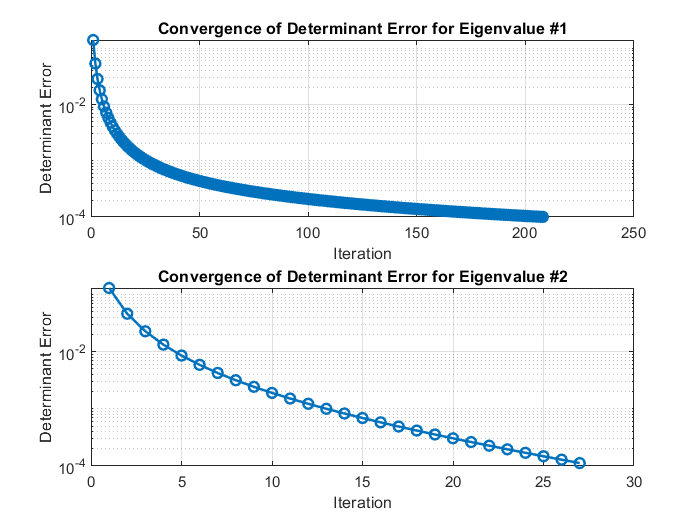
\includegraphics[width=0.8\linewidth]{Figures/eigen_value_exact.png}
        \caption{Illustrating the convergence of determinant errors for two eigenvalues across iterations}
        \label{fig:enter-label}
    \end{figure}
\end{center}

\newpage
The graphical representation captures the convergence behavior of determinant errors associated with two distinct eigenvalues across a series of iterative steps.  This graph provides valuable insights into the iterative refinement process, illustrating how the determinant error diminishes over successive iterations, thus indicating the improving accuracy and convergence of the eigenvalue computations for the given matrix.